\begin{figure*}[t]
  \centering
  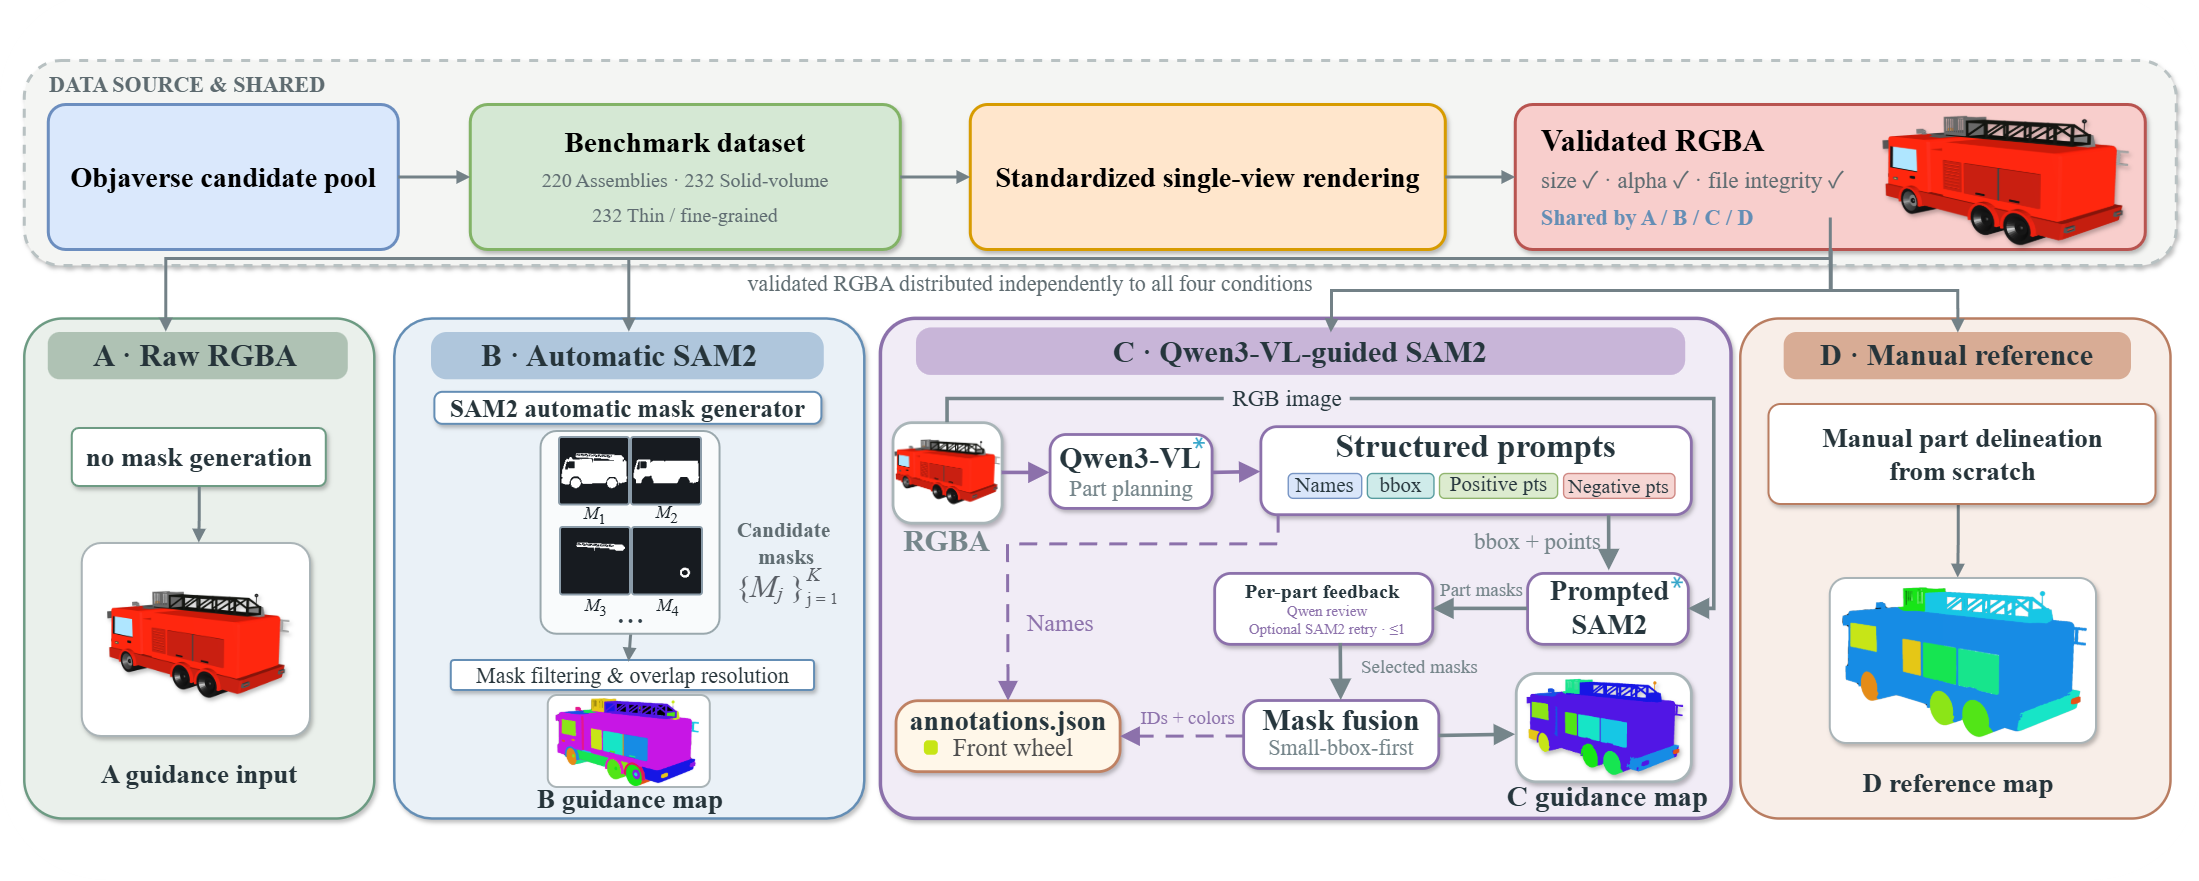
\includegraphics[width=\textwidth]{images/fig2_data.png}
  \caption{数据处理与四种引导条件。基准候选集按结构特征划分为 220 个组装结构、232 个实体体积结构和 232 个细薄／细粒度结构对象。A 使用原始 RGBA；B 从自动 SAM2 候选中筛选并处理重叠；C 使用部件规划、空间提示、候选反馈及小框优先融合，同时保存名称与二维标签的对应关系；D 为人工直接制作并渲染的二维部件参考，不来自 B 的自动结果修补，也不等同于完整三维真值。图内 D 的 ``from scratch'' 仅用于区别自动分支，具体人工制作流程仍需在数据说明中补全。C 的反馈在候选掩码阶段执行，每个被判为需要修正的候选至多重试一次。}
  \label{fig:data}
\end{figure*}
